\documentclass[]{nrel} 
%%%%%  Package options place in square brackets
% singleAppendix -- format TOC and appendix chapters without lettering
% draft -- add watermark "draft"
% confidential -- change footer to state contents are confidential

\usepackage{hyperref}
\usepackage{listings}
\usepackage{xcolor}

\definecolor{codegreen}{rgb}{0,0.6,0}
\definecolor{codegray}{rgb}{0.5,0.5,0.5}
\definecolor{codepurple}{rgb}{0.58,0,0.82}
\definecolor{backcolour}{rgb}{0.95,0.95,0.92}

%\lstdefinestyle{mystyle}{
%    backgroundcolor=\color{backcolour},   
%    commentstyle=\color{codegreen},
%    keywordstyle=\color{magenta},
%    numberstyle=\tiny\color{codegray},
%    stringstyle=\color{codepurple},
%    basicstyle=\ttfamily\footnotesize,
%    breakatwhitespace=false,         
%    breaklines=true,                 
%    captionpos=b,                    
%    keepspaces=true,                 
%    numbers=left,                    
%    numbersep=5pt,                  
%    showspaces=false,                
%    showstringspaces=false,
%    showtabs=false,                  
%    tabsize=2
%}

%\lstset{style=mystyle}

% -----------------------------------
% DOCUMENT PROPERTIES
% -----------------------------------
\title{Research Software Best Practices}

\author{Rafael Mudafort} %<--------- Your name here
%\author{Author two} %<--------- Coauthor's name here
\affil{National Renewable Energy Laboratory}
%%%%% %<--------- If including authors from multiple institutions, the affiliation number each author needs to be 
% \author[1]{Author one}  %<--------- other NREL authors
% \affil[1]{National Renewable Energy Laboratory}
% \author[2]{Author two} %<--------- External collaborator
% \affil[2]{Another affiliation} %<--------- External collaborator affil

\fancypagestyle{plain}{}
%\addbibresource{refs.bib}  %<--------- add bibliographic items to this file
\setcounter{tocdepth}{2}
% -------------------------------------
% DOCUMENT STARTS HERE
% -------------------------------------
\begin{document}


\frontmatter
%%%%%%%%%%%%%%%%%%%%%%%%%%%
%\chapter{Acknowledgments}
% <text>

% %%%%%%%%%%%%%%%%%%%%%%%%%%% 
% \chapter{Acronyms} %<--------- Uncomment this section if adding acronyms
% \acro{DOE}{Department of Energy}

%%%%%%%%%%%%%%%%%%%%%%%%%%%
\chapter{Executive Summary}
% <text>

Wind energy researchers typically share one key characteristic: a passion for increasing
wind energy in the global energy mix. The U.S. Department of Energy (DOE) supports this mission
in a number of ways including allocating funding directly to various aspects of wind energy
research through the
\href{https://www.energy.gov/eere/office-energy-efficiency-renewable-energy}{Office of Energy Efficiency and Renewable Energy (EERE)}
via the
\href{https://www.energy.gov/eere/wind/wind-energy-technologies-office}{Wind Energy Technologies Office (WETO)}.
While the traditional output of research is academic publication, software development efforts
are increasingly a major focus. Software tools in the research environment allow researchers to
describe an idea and quickly increase the scope and scale as they study it further.
As a product of research, these tools represent a direct pipeline from researcher to industry
practitioners since they are the implementation of ideas described in academic publications.
Given this vital role in wind energy research and
commercial development, the broad research software portfolio supported by WETO must maintain a
minimum level of quality to support the wind energy field in the growing transition to
renewable energy. \textbf{This report outlines a series of best practices to be adopted by all
WETO-supported software projects, as well as expectations that the communities interacting with
these projects should have of the developers and tools themselves.}

Wind energy research software has a unique standing in the field of scientific software. The
stakeholders are varied with a subset being:


\begin{itemize}
\item DOE EERE leadership

\item DOE WETO leadership and program managers

\item National lab leadership

\item Associated project principle investigators

\item Research software engineers

\item Wind energy researchers in academia
(including graduate students, post docs, and national lab staff)

\item Industry researchers and practitioners

\item Commercial software developers

\item The general public interested in wind energy

\end{itemize}

These software are typically the end-user of other generic software libraries, so
the funding cycles are often tied to applied research rather than the development of the
software itself. Since the developers are also wind energy researchers, these tools are
typically designed in a way that closely resembles the application in which they’re used.
Additionally, the expertise and incentives for the developers have a high variability, and
often neither are aligned with software engineering or computer science.

Given the unique environment in which wind energy research software is produced and consumed,
it is critical for model owners to understand the context of their software. A framework
for developing this understanding is to answer the following questions of a given software project:
\begin{itemize}
\item What is it’s purpose?

\item What is it’s role in the field of wind energy?

\item What is the profile of the expected users?

\item For how long will it be relevant?

\item What is the expected impact?

\end{itemize}

These questions allow model owners to identify the appropriate methods for the design, development,
and long term maintenance of their software. Additionally, the answer provide context for future
planners to understand why particular decisions were made and discern the consequences of
changing course.

The information is aggregated from experience within WETO-supported software development
groups as well as external organizations and efforts to define the craft of research software
engineering. These best practices aim to make the collaborative development process efficient
and effective while improving the model understanding across stakeholders. Additionally,
the general adoption of a common framework for software quality ensures that the end users
of WETO software can trust these tools and accurately understand the risks to workflow integration.


\clearpage
\tableofcontents
\listoffigures
%\listoftables

\mainmatter
\pagestyle{fancy}




\chapter{Summary of best practices}

\nameref{sec:accessibility}
\begin{itemize}
\item Determine the barriers to entry for expected users and address accessibility accordingly.
Automate accessibility methods and processes so that it is implicit in the software
development process.

\item Prerequisite knowledge - Identify target user profiles and anticipate their levels of understanding.
Accurately understand the complexity of the systems used to access the software, and evaluate
whether this matches the expected skills in target users.
Note that technical solutions can be augmented with documentation to address gaps in prerequisite
knowledge.

\item Distribution - Provide a streamlined method of installation using common software distribution systems.
\end{itemize}

\nameref{sec:usability}
\begin{itemize}
\item User interface - UIs should be predictable, and adopt existing conventions for the contexts
in which they exist.

\item Command line interface - If a CLI exists, it should be meaningful, predictable, and well documented.
Refer to contextual guidelines and conventions for flags, syntax, and functionality.
At a minimum, provide documentation via the help flag, and extended documentation alongside
examples and tutorials is helpful.

\item Input and output files - Use a common file structure relevant to the type of data produced from a software,
and leverage the existing ecosystem of tools to pre and post-process input and output files.

\item Error messages - Identify an error messaging system that enables communicating to users without encumbering
the development process.
Provide useful errors that include data, provide guidance for moving forward, and help maintainers
identify potential bugs.

\item Metadata - Providing metadata to users requires minimal effort for developers, and it enables users to more
effectively share and compare data and get help. At a minimum, display version numbers, critical
settings, and dependency info.
\end{itemize}

\nameref{sec:extendability}
\begin{itemize}
\item How easily a project can be extended is critical to it's viability as a long term
DOE-funded project.
Prioritize simplicity in architecture, dependencies, and toolchains.
Create a development environment balancing modern needs with stability.
\item Code style - Strive to write code that external developers can easily read and comprehend with minimal
preexisting context.
\item Architecture and design - Adopt an explicit design process where the major ideas are made chosen prior to writing any code.
\item Software design process - Create a parti and list performance requirements for each level of fidelity in the software.
Establish methods to validate the design and implementation given knowledge of how a software
is ultimately used.
\item Design patterns - Study existing design patterns, and adopt a few, as needed.
Refer to existing materials especially relevant to research software architecture.
\item Version control - Craft a version control history that communicates the evolution of changes of the software
to future developers including the author of current changes.
Evolve the software in a logical, linear process with digestible, easily reviewable changes.
\item Collaborative workflows with GitHub - Treat GitHub as the home page of a software project, and develop the planning and coordination
activities as a first-order communication, signalling, and organizational mechanism for the
community of users.
\item Pull Requests - All components of a pull request should be considered documentation for future reference
and an aspect of version control.
PR reviews should be verbose, thorough, positive, and referential to guiding documents.
\item Continuous integration: automating tests, compliance, and delivery - Codify software quality by establishing automated systems to check and provide feedback
within the development process.
Offload as many manual processes as possible and practical to the continuous integration system.
\end{itemize}


\chapter{Accessibility}
\label{sec:accessibility}

Accessibility is concerned with how practitioners are expected to obtain and integrate a software
into their processes. The product that is to be obtained is the executable version of the software.
In the case of compiled programming languages, this is a binary executable or library file,
while interpreted languages typically require distributing the source code directly.

For guidance on developer accessibility, see \nameref{sec:extendability}.

The technical approaches to address accessibility depend on the targeted users.
To identify methods for improving accessibility, first identify the expected users and
anticipate their barriers to entry.
Then, create processes and technical solutions to minimize these barriers.
Finally, automated the processes so that accessibility is implicit to the process rather than
dependent on developers remembering to meet these needs.

\section{Prerequisite knowledge}

Using a computer in a scientific context is a learned skill and requires years of practice to
become proficient. Tools like a "terminal", "shell", or "command prompt" are not universally
intuitive, and that these three terms are used interchangeably can lead to further confusion.
This is an example of a barrier to entry often encountered by early-career researchers and
experienced practitioners alike. In order to improve accessibility, it is important to
understand the experience of users and design software to meet their needs.

Some examples of common barriers to entry are:
\begin{itemize}
\item Navigating a "terminal"

\item Knowledge of acronyms, jargon, or interchangeable phrases
\begin{itemize}
\item CLI, API, IDE, etc

\item Compile, clone, check out

\item Terminal vs shell vs command prompt

\end{itemize}

\item Extensions: \lstinline{.exe}, \lstinline{.so}, \lstinline{.dll}, \lstinline{.dylib}

\item Installation:
\begin{itemize}
\item Package managers

\item Downloading executable files

\item Configuring an environment

\end{itemize}

\end{itemize}

Identify target user profiles including their levels of experience of understanding in
computing environments.
Then, design the research software so that it matches the expected level of expertise in
users.
Note that this is often an iterative process, and technical solutions are not always needed
to address barriers to entry.
Explanatory documentation is a major resource in addressing ambiguity or inexperience in
a particular technology.
Leverage existing tutorials were necessary; for example, a high-level overview of methods
to use a terminal in the context of a specific software project along with an accompanying
link to a deep dive into terminal training can be very helpful.

\section{Distribution}

Research computing software often depend on third-party libraries, and many of these dependencies
are research software themselves. Therefore, the installation and environment configuration
for this type of software can easily become complex.
Mature package managers are a great resource since they have a distribution system already in place
and manage dependencies between software tools.
The ecosystem of open source software package managers has coalesced around a few primary tools:
\begin{itemize}

\item \href{https://pypi.org}{Python Package Index (PyPI)}
\begin{itemize}
\item Source and binary distribution package manager for Python software
\item Platform: any
\end{itemize}

\item \href{https://docs.conda.io/en/latest/}{Conda}
\begin{itemize}
\item Package, dependency and environment management for any language
\item Platform: any
\end{itemize}

\item \href{https://conda-forge.org}{Conda-forge}
\begin{itemize}
\item A community-led collection of recipes, build infrastructure and distributions for the conda package manager
\item Platform: any
\end{itemize}

\item \href{https://brew.sh}{Homebrew (brew)}
\begin{itemize}
\item The Missing Package Manager for macOS (or Linux)
\item Platform: Ubiquitous for macOS, but also available for Linux
\end{itemize}

\item \href{https://spack.io}{Spack}
\begin{itemize}
\item Spack is a package manager for supercomputers supporting any language and distributable product
\item Platform: Ubiquitous for Linux-based supercomputers, and also available for macOS and Linux
\end{itemize}

\item \href{https://en.wikipedia.org/wiki/APT\_(software)}{APT}
\begin{itemize}
\item A user interface that works with core libraries to handle the installation and removal of software on Debian, and Debian-based Linux distributions
\item Platform: Ubiquitous for Linux for system-level or generic packages
\end{itemize}

\item \href{https://fpm.fortran-lang.org/index.html}{Fortran package manager (FPM)}
\begin{itemize}
\item Fortran-specific executable and library package manager.
\end{itemize}

\end{itemize}

The process for including a package in a package management system varies, but all are designed
to integrate with automated systems to prepare and distribute the package automatically upon
a given event. The practice of releasing a software package after a tagged release
(see \nameref{sec:version_control}) or requisite set of changes is called "continuous distribution",
a component of "continuous integration". See \nameref{sec:continuous} for details.
Tools for this level of automation are ubiquitous, and a practical choice
is GitHub Actions (see \nameref{sec:github}).


\chapter{Usability}
\label{sec:usability}
Usability is concerned with how practitioners are expected to execute the software including
creating inputs and managing outputs.
While the content and promise of a particular software will bring users to it in the first
place, the ease of usability is responsible for keeping them engaged with the software.
In this context, consider any user interfaces including messaging back to the user through
errors as the "touch points" that should be optimized.
Developers should recall their own experience in using software including outside
of the research environment.
Contemporary software consumers have short attention spans and will generally choose
the path of least resistance to accomplish a task even at the cost of access to a more
advanced feature.

\section{User interface}
The user interface (UI) is any mechanism through which users interact with the software
typically by providing inputs and receiving outputs. Examples of UI's include:

\begin{itemize}
\item Graphical user interface (GUI)
\item Web-based front ends
\item Input and output files
\item Command line interface
\item Library API's
\end{itemize}

WETO software UI's should be well defined and predictable.
They should adopt the conventions that already exist in the environments and contexts
in which they're used.
Most importantly, all user interfaces should be well documented.

\subsection{Command line interface}
The command line interface (CLI) is one type of front-end for software.
It is the method by which a software is executed via a computer’s terminal.
WETO software should in general adhere to the following conventions and principles for CLI’s.
However, these are guidelines and can be skipped when context is clear or another
option improves usability.

\begin{itemize}
\item Adopt command line syntax requirements from \url{https://pubs.opengroup.org/onlinepubs/9699919799/basedefs/V1\_chap12.html}
\begin{itemize}
\item Guideline 1: Utility names should be between two and nine characters, inclusive.
\item Guideline 2: Utility names should include lowercase letters (the lower character classification) and digits only from the portable character set.
\item Guideline 3: Each option name should be a single alphanumeric character (the alnum character classification) from the portable character set. The \lstinline{-W} (capital-W) option shall be reserved for vendor options. Multi-digit options should not be allowed.
\item Guideline 4: All options should be preceded by the `-`` delimiter character.
\item Guideline 5: One or more options without option-arguments, followed by at most one option that takes an option-argument, should be accepted when grouped behind one \lstinline{-} delimiter.
\item Guideline 6: Each option and option-argument should be a separate argument, except as noted in \href{https://pubs.opengroup.org/onlinepubs/9699919799/basedefs/V1\_chap12.html}{Utility Argument Syntax, item (2)}.
\item Guideline 7: Option-arguments should not be optional.
\item Guideline 8: When multiple option-arguments are specified to follow a single option, they should be presented as a single argument, using \lstinline{<comma>} characters within that argument or \lstinline{<blank>} characters within that argument to separate them.
\item Guideline 9: All options should precede operands on the command line.
\item Guideline 10: The first \lstinline{--} argument that is not an option-argument should be accepted as a delimiter indicating the end of options. Any following arguments should be treated as operands, even if they begin with the \lstinline{-} character.
\item Guideline 11: The order of different options relative to one another should not matter, unless the options are documented as mutually-exclusive and such an option is documented to override any incompatible options preceding it. If an option that has option-arguments is repeated, the option and option-argument combinations should be interpreted in the order specified on the command line.
\item Guideline 12: The order of operands may matter and position-related interpretations should be determined on a utility-specific basis.
\item Guideline 13: For utilities that use operands to represent files to be opened for either reading or writing, the \lstinline{-} operand should be used to mean only standard input (or standard output when it is clear from context that an output file is being specified) or a file named "-".
\item Guideline 14: If an argument can be identified according to Guidelines 3 through 10 as an option, or as a group of options without option-arguments behind one \lstinline{-} delimiter, then it should be treated as such.
\end{itemize}

\item Adopt these minimum GNU conventions
\begin{itemize}
\item A short version with one dash and a long version with two dashes
\item \lstinline{-v} / \lstinline{--version} to show version information
\item \lstinline{-h} / \lstinline{--help} to display help information
\item \lstinline{-i} / \lstinline{--input} for input file specification
\item \lstinline{-o} / \lstinline{--output} for input file specification
\item \lstinline{-V} / \lstinline{--verbose} to include additional output in terminal
\item \lstinline{-q} / \lstinline{--quiet} to suppress terminal output
\end{itemize}

\item Use context-specific switches
\begin{itemize}
\item Unix: \lstinline{-} or \lstinline{--}
\item Python: \lstinline{-} or \lstinline{--}
\item Windows command prompt: \lstinline{/}
\end{itemize}

\end{itemize}

Command line interfaces should include documentation via the \lstinline{--help} / \lstinline{-h} flag.
For Python software, using the standard \href{https://docs.python.org/3/library/argparse.html}{argparse}
library creates a help prompt automatically.
Extended CLI documentation alongside tutorials and explanations of the software is helpful to
attach meaning to the functionality available via the CLI.

\subsection{Input and output files}
The ecosystem of tools for processing data files is vast and mature.
Therefore, input and output files should adopt a common file type and syntax relevant to the
field and context of the software itself.
For example, large datasets generated by computational fluid dynamics software are often
exported in \href{https://www.hdfgroup.org/solutions/hdf5/}{HDF5} format since robust
libraries are available to export the data and load it into post-processing tools.
Similarly, input files should retain a ubiquitous human-readable format such as
\href{https://yaml.org}{YAML} as this allows users to generate input files programmatically
using standard libraries. Input and output files required by WETO software should
adhere to the following conventions and principles:

\begin{itemize}
\item Simple, clear, and predictable structure
\item Expressive and concise
\item Easy to produce and consume using ubiquitous software tools

\item Minimal data consumption
\begin{itemize}
    \item For large data sets, option to split into smaller files or binary format
\end{itemize}

\item Typical and predictable data types
\begin{itemize}
\item For large data sets, option to split into smaller files or binary format
\end{itemize}

\end{itemize}

File types with common libraries for popular language ecosystems are:
\begin{itemize}
\item \href{https://developer.mozilla.org/en-US/docs/Learn/JavaScript/Objects/JSON}{JSON} - JavaScript
    Object Notation; a very common data structure used throughout the web and in various
    computing environments
\item \href{https://yaml.org}{YAML} - YAML Aint Markup Language; not entirely but basically a
    human-readable version of JSON
\item \href{https://en.wikipedia.org/wiki/Comma-separated_values}{CSV} - Comma separated values
\item \href{https://examples.vtk.org/site/VTKFileFormats/}{VTK} - Visualization Tool Kit; a variety of
    file types and readers for different types of data
\item \href{https://portal.hdfgroup.org/display/HDF5/HDF5}{HDF5} - Hierarchical Data Format; used for large,
    complex, heterogeneous data sets; HDF includes libraries for reading and writing HDF files
\item \href{https://github.com/nasa/Plot3D_utilities}{Plot3D} - Data type for 3D structured grid data
\item \href{https://cgns.github.io/WhatIsCGNS.html}{CGNS} - CFD General Notation System
\item \href{https://www.markdownguide.org/getting-started/}{Markdown} - A markup language for text documents
\item \href{https://docutils.sourceforge.io/rst.html}{reStructured Text} - A markup language for text
    documents
\end{itemize}

\section{Error messages}
Messaging to practitioners from within a software can be immensely helpful.
At the same time, the infrastructure for communicating messages can be a heavy lift.
It is important to find a balance of appropriate levels of messaging while also ensuring that
the messages themselves are up to date with the software features and implementations.
Too much messaging results in information overload and critical messages can be lost in noise.
Additionally, messaging is another developer responsibility and can be overlooked among all of the
other responsibilities during the development cycle.

\begin{itemize}

\item Expect that the reader does not have the context of the author
\begin{itemize}
\item Include a stack trace in all messages
\item At minimum, include the calling function name
\end{itemize}

\item Anticipate the needs of the reader
\begin{itemize}
\item What will they be thinking about when this error pops up?
\item What will they need to do next?
\end{itemize}

\item Include information that will help project maintainers understand the context of the problem
\begin{itemize}
\item Include metadata where relevant; see \nameref{sec:metadata}
\item Include the value of data that is found invalid
\end{itemize}

\end{itemize}


\section{Metadata}
\label{sec:metadata}
Tracking metadata in software projects is a simple way to provide clarity to all users.
This greatly improves usability and has the added effect of improving the debugging process.
This information can be provided to the user in any structured output from the software.
For example, output data files, reports, images, etc can all include a snapshot of the metadata.
The objective is to communicate information on the state of the software (version and runtime),
the state of the computing environment, and any user decisions.

The following fields are minimum metadata to include:
\begin{itemize}
\item Version number in \href{https://semver.org}{semantic versioning format} (MAJOR.MINOR.BUGFIX, i.e. v3.2.1)
\item Execution time

\item Compile info, if applicable
\begin{itemize}
\item Compiler vendor
\item Compile time
\item Compiler settings
\end{itemize}

\item System information such as OS, relevant hardware (i.e. accelerators) vendor
\item Relevant settings enabled

\end{itemize}


\chapter{Extendability}
\label{sec:extendability}
Extendability is concerned with how improvements such as new features, bug fixes, and general
maintenance are added to an existing software project. This covers both the technical aspects
as well as the management of multiple developers and development efforts happening
concurrently.

The lifecycle of WETO software projects typically follows a pattern of funding,
development, and release resulting in a recurring development workflow depicted in Figure \ref{fig:dev_lifecycle}.
The "Maintenance" tasks are usually optional and implicitly embedded
in future development efforts. Therefore, it is critical to the life of all WETO software to
prioritize extendability so that future funding opportunities are attractive to stakeholders,
and general maintenance and infrastructure upgrades can be introduced with minimal overhead.

\begin{figure}[htbp]
\begin{center}
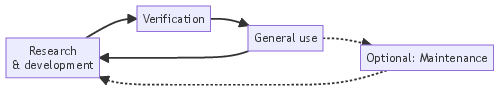
\includegraphics[width=0.7\textwidth]{mermaid-d1bafe392e85b8f467e3d93074dc8d7b7c45dfd0.png}
\caption{A representation of the typical lifecycle of software extension tasks within the research environment.}
\label{fig:dev_lifecycle}
\end{center}
\end{figure}

% This topic is closely tied to \nameref{communicating_design}, and the objective is to ensure that
This topic is closely tied to the need for communicating elements of design, and the objective is to ensure that
developers can easily approach the project with minimal overhead required to align their
computing environment, scope the work, implement the changes, and verify the results.

A guiding principle on extendability is to use ubiquitous infrastructure.
Mature and ubiquitous tools and libraries come with formal and community-based documentation,
ecosystems of tools such as IDE extensions, and institutional or cultural knowledge of
their use and nuances that can be difficult and time consuming to create for specialized
infrastructure.
Common build systems such as CMake with the GNU or LLVM toolchains should be used instead of
the newest projects.
Popular programming languages (Python, C++, Fortran) are more approachable than specialized
languages (Rust, Julia, Elixir), and enable a wider developer base.
Software project managers should strive to create a development environment balancing the need for
modern tooling, modern developer expectations, and stability.

\section{Code style}
In software development, the word "grok" is often used (see usage in
\href{https://hn.algolia.com/?q=grok}{Hacker News},
\href{https://lobste.rs/search?q=grok\&what=stories\&order=newest}{Lobsters},
\href{https://stackoverflow.com/search?tab=newest\&q=grok\&searchOn=3}{StackOverflow})
to communicate about degrees of understanding. This word is described by it’s creator below
(Source: \href{https://en.wikipedia.org/wiki/Grok}{Wikipedia}).
\begin{quote}

\textit{Grok} means "to understand", of course, but Dr. Mahmoud, who might be termed the leading
Terran expert on Martians, explains that it also means, "to drink" and "a hundred other
English words, words which we think of as antithetical concepts. ‘Grok’ means \textit{all} of
these. It means ‘fear’, it means ‘love’, it means ‘hate’ – proper hate, for by the Martian
‘map’ you cannot hate anything unless you grok it, understand it so thoroughly that you
merge with it and it merges with you – then you can hate it. By hating yourself. But this
implies that you love it, too, and cherish it and would not have it otherwise. Then you
can \textit{hate} – and (I think) Martian hate is an emotion so black that the nearest human
equivalent could only be called mild distaste.
\end{quote}

That such a word exists and is widely used in software development illustrates the high value
of clear and understandable code.
WETO software should avoid complexity where possible and favor readability over writability.
Strive to create software that can be easily grokked by developers who do not have the current
context, and remember that often these developers are domain experts rather than
computer scientists.

The designers of the Python programming language consider readability as a primary priority, and
the most famous of the many Python language-development documents is
\href{https://peps.python.org/pep-0008/}{PEP 8} which proposes a style guide for Python code.
PEP 8 is summarized into 19 aphorisms (20 including one that’s implied) and is referred to as
\href{https://peps.python.org/pep-0020/}{"The Zen of Python"}. Much of the WETO software portfolio is
Python-based, so these guiding principles directly apply. However, these principles are
programming language agnostic and eloquently describe the paradigm for developing
extendable software.


\subsection{The Zen of Python}
\label{sec:zen}

\begin{lstlisting}[language=Python]
import this
\end{lstlisting}

\begin{lstlisting}
The Zen of Python, by Tim Peters

Beautiful is better than ugly.
Explicit is better than implicit.
Simple is better than complex.
Complex is better than complicated.
Flat is better than nested.
Sparse is better than dense.
Readability counts.
Special cases aren't special enough to break the rules.
Although practicality beats purity.
Errors should never pass silently.
Unless explicitly silenced.
In the face of ambiguity, refuse the temptation to guess.
There should be one -- and preferably only one -- obvious way to do it.
Although that way may not be obvious at first unless you're Dutch.
Now is better than never.
Although never is often better than *right* now.
If the implementation is hard to explain, it's a bad idea.
If the implementation is easy to explain, it may be a good idea.
Namespaces are one honking great idea -- let's do more of those!
\end{lstlisting}

\section{Architecture and design}

\begin{quote}
    If you think good architecture is expensive, try bad architecture.

    -- Brian Foote and Joseph Yoder, Clean Architecture: A Craftsman's Guide to Software Structure and Design
\end{quote}

In the development of any complex system, the design and it's implementation are either
explicit or implicit.
Explicit design involves identifying relationships between modules, composition of data
structures, and flow of data prior to writing code, whereas an implicit design evolves during the
process of writing new code.
In open source software, an explicit design process is critical to allowing the project
to grow beyond a single developer, and the consequence of an implicit design process
is the common case of technical debt.

\subsection{Software design process}

Primarily, an explicit design process involves identifying the fundamental principles
of a particular design - how it is expected to function in various aspects.
This process should result in two statements:

\begin{enumerate}
\item The \href{https://en.wikipedia.org/wiki/Parti_(architecture)}{parti}, a description of the
    fundamental, driving design intent as a brief text (one or two sentences) or a
    simple diagram
\item A list of requirements that the parti and it's implementation should satisfy
\end{enumerate}

The \textit{parti} is the abstract objective and the list of requirements are the criteria
to verify that the implementation satisfies the parti.
In other words, these are the tests for the design.
Upon establishing this information, it should be codified into a design document and style
guide that are made publicly available to all developers such as in online documentation.

There are various levels of fidelity to consider when designing a software system:
\begin{itemize}
\item Level 0: Syntax and code style
\item Level 1: Function scope, function signatures
\item Level 2: Module composition
\item Level 3: System composition
\end{itemize}

Each should be addressed individually but referring to each other. For example, having a major
design driver to limit complexity at Level 3 can be negated if complexity is allowed
at Level 0. However, the definition of complexity at these levels are entirely different and
should be directly defined.

\begin{quote}
    Architecture is a hypothesis that needs to be proven by implementation and measurement

    -- Tom Gilb, Clean Architecture: A Craftsman's Guide to Software Structure and Design
\end{quote}

While having an explicit design process is important, it is not required to stick to a chosen
design at all cost.
Throughout the development of a software, the architecture and design should be regularly
revisited and reevaluated given the new knowledge acquired during implementation.
How a software is ultimately used and the problems faced cannot be known at design time,
so developing a process for design validation is required.

\subsection{Design patterns}
The software engineering community has created a wide range of
\href{https://en.wikipedia.org/wiki/Software_design_pattern#Classification_and_list}{design patterns}
to address specific design problems.
These are often used as a reference for creating a specific architectural design,
and they often focus on fidelity levels 1 and 2.
Multiple design patterns can even be pieced together to create a high-level monolithic architecture.
The benefits of adopting an existing design pattern are:
\begin{itemize}
    
    \item The methods to describe the design pattern to new developers are already established
    \item Teams can work with the architecture in the abstract to develop their concrete customized
        implementation
    \item Ecosystems of third-party tools exist to leverage some of the common design patterns
    \item Some patterns can be easily replaced by others \textit{in situ}
\end{itemize}

While software architecture and software design patterns are entire fields of knowledge,
many resources exist to teach common methods.
A few in depth references specifically relevant to WETO-supported research software are:
\begin{itemize}    
\item Uncle Bob's \href{https://books.google.com/books/about/Clean_Architecture.html?id=uGE1DwAAQBAJ&source=kp_book_description}{Clean Architecture: A Craftsman's Guide to Software Structure and Design}
\item \href{https://www.youtube.com/watch?v=UWmkj-9SdAI}{IDEAS-ECP HPC Best Practices Webinar: Software Design Patterns in Research Software with Examples from OpenFOAM}
\item Architecture of Open Source Applications \href{https://aosabook.org/en/#aosa1}{Volume 1} and \href{https://aosabook.org/en/#aosa2}{Volume 2}
\end{itemize}


\section{Version control}
\label{sec:version_control}

Version control, typically with \href{https://git-scm.com}{git}, is a tool for tracking the
evolution of a project change by change establishing a history of changes.
Each change, called a "commit", is itself a version of the software, and, collectively,
the changes provide a snapshot of thought processes and progression of work.

Version control with git can seem like simply a mechanism to "save" the state of a document,
and it is easy to relegate this process to a secondary concern in the development process.
However, it carries far more meaning in the context of software extendability.
Since the git system is decentralized, it allows multiple developers to make changes to a
project concurrently.
Git also provides a mechanism for resolving differences so that multiple changes can be merged
together easily.

In addition to the content of changes themselves, the connectivity between changes over the
lifetime of a project is meaningful.
The connectivity between commits is structured as a
\href{https://en.wikipedia.org/wiki/Directed\_acyclic\_graph}{directed acyclical graph (DAG)}.
Each commit has a parent and each parent can have multiple children.
This provides a mechanism for easily and accurately rolling back to the state of the project at any
time in history.

To best leverage the power of git to enable extendability, consider the following guidelines:
\begin{itemize}
\item It is reasonable to spend time crafting each commit and a sequence of commits.
\item Each commit should optimize for readability in both the content of the changes and the message
\begin{itemize}
    \item Keep changes within an easily communicated scope
    \item Avoid the temptation to mix formatting changes with algorithmic changes
    \item More smaller commits are generally better than fewer large commits
\end{itemize}
\item Practice editing a series of commits to ensure that the progress of work is captured accurately.
\item Consider whether the commit history is concise and readable to people who are not the authors.
\item Become familiar with the following actions:
\begin{itemize}
    \item Interactive rebase
    \item Cherry-pick
    \item Squash
    \item Edit a commit message
\end{itemize}
\item Commit messages should be short, and it is a convention to limit them less than 50 characters.
\item An additional line can be included as a longer description of the commit beneath the
50 character line. The second line is typically limited to 70 characters, but it is
considered reasonable to use as much space as needed.

\end{itemize}


\section{Collaborative workflows with GitHub}
\label{sec:github}

The processes through which developers interact with a software and other developers is
an essential component of extendability.
These processes should generally strive for efficiency while minimizing overhead.
Automated processes are better than manual processes, and objective is better than subjective.
The majority of collaborative software development processes occur on the
\href{https://github.com}{GitHub} platform and automated processes leverage GitHub's free
cloud-based resources.

GitHub and git (see \nameref{sec:version_control}) are tightly connected, but they are different
systems and serve different purposes in the development process.
Git is a version control system for tracking and merging changes to a software.
GitHub is a platform for orchestrating and coordinating the various processes that happen
around the development cycle.
GitHub activities add context on top of the individual changes captured in commits.
Whereas commits often capture low-level information, GitHub activities can map the low level
details to high-level efforts.
GitHub provides extensive \href{https://docs.github.com/en/get-started/quickstart/git-and-github-learning-resources}{training material}
for git as well as GitHub features.

The primary GitHub features are described below, and a typical sequence of events across these
features is diagramed in Figure \ref{fig:dev_sequence}.

\begin{itemize}
\item \href{https://github.com/features/actions}{Actions}: This is a full-featured cloud computing
environment that is typically used for automating software quality processes such as
running tests, compiling software for release and distribution, and compiling and deploying
online documentation.

\item \href{https://docs.github.com/en/discussions}{Discussions}: This is typically the starting point
for any collaboration. Create a discussion topic and engage with other model stakeholders
to define the idea and develop a proposed implementation.

\item \href{https://docs.github.com/en/issues/tracking-your-work-with-issues/about-issues}{Issues}:
Document the proposed solution to a problem or implementation of a new feature as outlined
in the corresponding Discussion. Finalize the description and outline test cases to verify
the idea.

\item \href{https://docs.github.com/en/issues/planning-and-tracking-with-projects/learning-about-projects/about-projects}{Projects}:
Collect Issues, Pull Requests, and generic cards to establish a relationship across all
ongoing works in progress. This is typically most useful for large development efforts
and prioritizing work for upcoming releases.

\item \href{https://docs.github.com/en/pull-requests/collaborating-with-pull-requests/proposing-changes-to-your-work-with-pull-requests/about-pull-requests}{Pull Requests}:
Pull Requests (PR) are a request to accept a change into a branch. This typically happens
across forks of a repository, but it can also happen between branches of the same fork.
During the implementation of an Issue, open a pull request to communicate that work is
ongoing. This is also the venue for code reviews.

\item \href{https://docs.github.com/en/repositories/releasing-projects-on-github/about-releases}{Releases}:
A number of accepted pull requests can be aggregated to comprise one release, and this is
listed in a project’s GitHub Releases page along with release notes to describe the changes
and communicate relevant details.

\end{itemize}

\begin{figure}[htbp]
\begin{center}
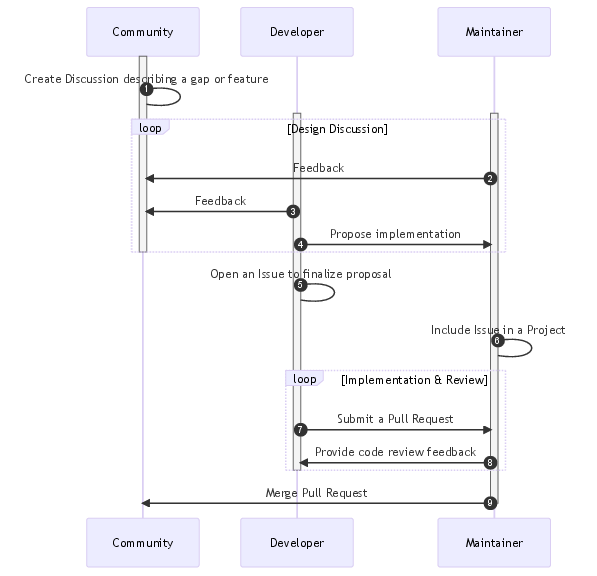
\includegraphics[width=0.8\textwidth]{mermaid-bfcb6a9556227d6b8158e111ddd0f37e43e4f635.png}
\caption{A representative workflow among all actors in a software development workflow leveraging GitHub features.}
\label{fig:dev_sequence}
\end{center}
\end{figure}

The combination of git and GitHub provides a powerful mechanism to capture design intent,
factors that lead to particular decisions, and the evolution of a project for future reference.
It is important carefully craft the messages to avoid washing out information with noise.
Consider the following guidelines when engaging on GitHub.

\begin{itemize}
\item Descriptions of any activity should be well scoped and easily understandable.
\item Pictures really are worth 1,000 words. Include a diagram, plot, screenshot, or picture
when it will add clarity.
\item Prefer actual text over of screenshots of text. GitHub is searchable, so text provides more
searchable content whereas screenshots do not. Additionally, text-based code snippets can be
copied easily by other users.
\item Establish a practice of assigning responsibility to a core team member for each Issue and
Pull Request to avoid ambiguity about how these will be addressed.

\end{itemize}


\section{Pull Requests}
A pull request, or "PR", is a request to merge a particular set of code changes into another
instance of the software, typically an agreed upon "main" version.
Pull request descriptions should include contextual information regarding the code change.
The objective is to convince reviewers and maintainers that the new code is in a good state,
and that it's inclusion would be a benefit to the project. This typically involves a contextual
description of the change, an explanation of why the change is valid, and an overview of the
tests added to the test suite to demonstrate and exercise the new code.

The size and scope of a pull request should be chosen so that it is both easy to explain and
easy to review.
It is common to create many pull requests in the development of a single
feature as this process enables periodically syncing forks or branches and supports
milestones or periodic check-ins throughout development.
The primary objective is to optimize for readability in the pull request description as well as
the code changes themselves.

Consider pull requests titles and descriptions as documentation that will be relevant to
future developers.
When a pull request is merged, it can either be combined into one commit (squash and merge)
in the destination branch or included through a merge-commit.
The former does not maintain the commit history of the working branch while the latter does.
The squash-and-merge approach is often preferred by project maintainers due to it's simplicity,
and in this case the title of the pull request becomes the commit message.
Since merging the pull request directly affects the commit history of the destination branch,
the review and merge process should also follow the \nameref{sec:version_control} guidelines.
Finally, the release process through GitHub Releases can automatically construct
release notes from the title of all pull requests merged since the previous release.

While the details of workflows around defining, designing, and implementing new development
efforts should be identified explicitly following the guidance in \nameref{sec:github}, pull requests,
in practice, are often a good place to iterate collaboratively on the design and implementation
details.
Pull request reviews should have the following characteristics:
- Be very verbose with efficient but specific and complete feedback
- Be constructive rather than destructive; blame (negative) is nearly always irrelevant,
    and credit (positive) is nearly always appreciated
- Call out good ideas as well as bad ideas
- Include snippets of code to exercise portions of the changes
- Include plots or graphics showing the impact of the changes
- Refer to precedent or contextual conventions
- Refer to design documentation and style guides

The \href{https://docs.github.com/en/pull-requests/collaborating-with-pull-requests/reviewing-changes-in-pull-requests/incorporating-feedback-in-your-pull-request}{GitHub Pull Request Review documentation}
provides a detailed guide on using the various features to suggest and integrate
code review feedback.


\section{Continuous integration: automating tests, compliance, and delivery}
\label{sec:continuous}

The term "continuous integration", or "CI", is often used to refer to any of the many
automated systems that support software quality.
In it's essence, continuous integration refers to the practice of deploying a change in
the code directly into the production or released version.
This practice is enabled by constructing a system of quality check infrastructure that gives
maintainers the confidence to accept a change and release immediately.
The "continuous" aspect refers to the automated nature of the quality check systems.
Ideally, full continuous integration requires that all characteristics and potential
impacts of a code change are tested and validated automatically and without human
input, such as:
\begin{itemize}
\item Requiring that new code is covered by unit tests, integration tests, and regression tests
\item Checking that impacts to computational cost (speed) are within a threshold
\item Checking that memory impacts are within a threshold
\item Validating documentation changes and functionality
\item Linting for code syntax
\end{itemize}

It can be helpful to break the topic of CI into three general areas:
\begin{itemize}
\item Continuous testing (CT)
\item Continuous compliance (CC)
\item Continuous delivery (CD)
\end{itemize}

Continuous testing is established by adopting a testing framework and ensuring that all
new code is well tested. While automatically testing the \textit{quality} of test may be impractical,
it is simple and helpful to automatically check the \textit{quantity} of tests to ensure that new
code is covered.
For the same of a user-friendly CT pipeline, consider grouping tests into categories
that can be run in parallel by the automated system.
Also, minimize the time required to execute the test suite so that developers get
the automated feedback as soon as possible.

Continuous compliance is related to automatically checking for code style, complexity,
existence of docstrings or other types of documentation, and any other requirements
that describe aspects of the code itself.
A common method is to use a linter for the programming language used.
Most linters are high configurable so it can be tailored to the needs and style of
the development team.
This step typically happens very quickly, so execution time is usually not a concern.

Continuous delivery handles how the software is exported to users for consumption.
For web-based software, this involves deploying to a server, whereas modeling and analysis
libraries are typically delivered via package managers or compiled binaries.
The "continuous" aspect of CD refers to the practice of automatically pushing the
"released" product upon any change to the primary branch or via a periodic semi-automated
release process.

All aspects of CI contribute to the quality of a software project, and a full ecosystem
of open source, freely available infrastructure is available to address them all.
Ultimately, though, the true beneficiary of CI pipelines are the developers and maintainers
since major portions of quality enforcement and distribution are automated.
Without this infrastructure, code reviews can be prohibitively time consuming and error prone,
and the release process can take hours or days.
By committing to the initial investment and regular maintenance, computers handle
these detailed and repetitive tasks.

Given the inherent challenges in managing groups of people with various software
development styles and opinions, establishing the automated systems described here
can help to align expectations around minimum standards for acceptance of code while
reducing the burden on a project's "benevolent dictator" or gatekeeper.
It is recommended to establish these processes at the onset of a software project, and
continuously adjust as needed.

For reference, a typical CI pipeline for a Python package is shown in Figure \ref{fig:ci_pipeline} below where the square
components are GitHub Actions steps.

\begin{figure}[htbp]
\begin{center}
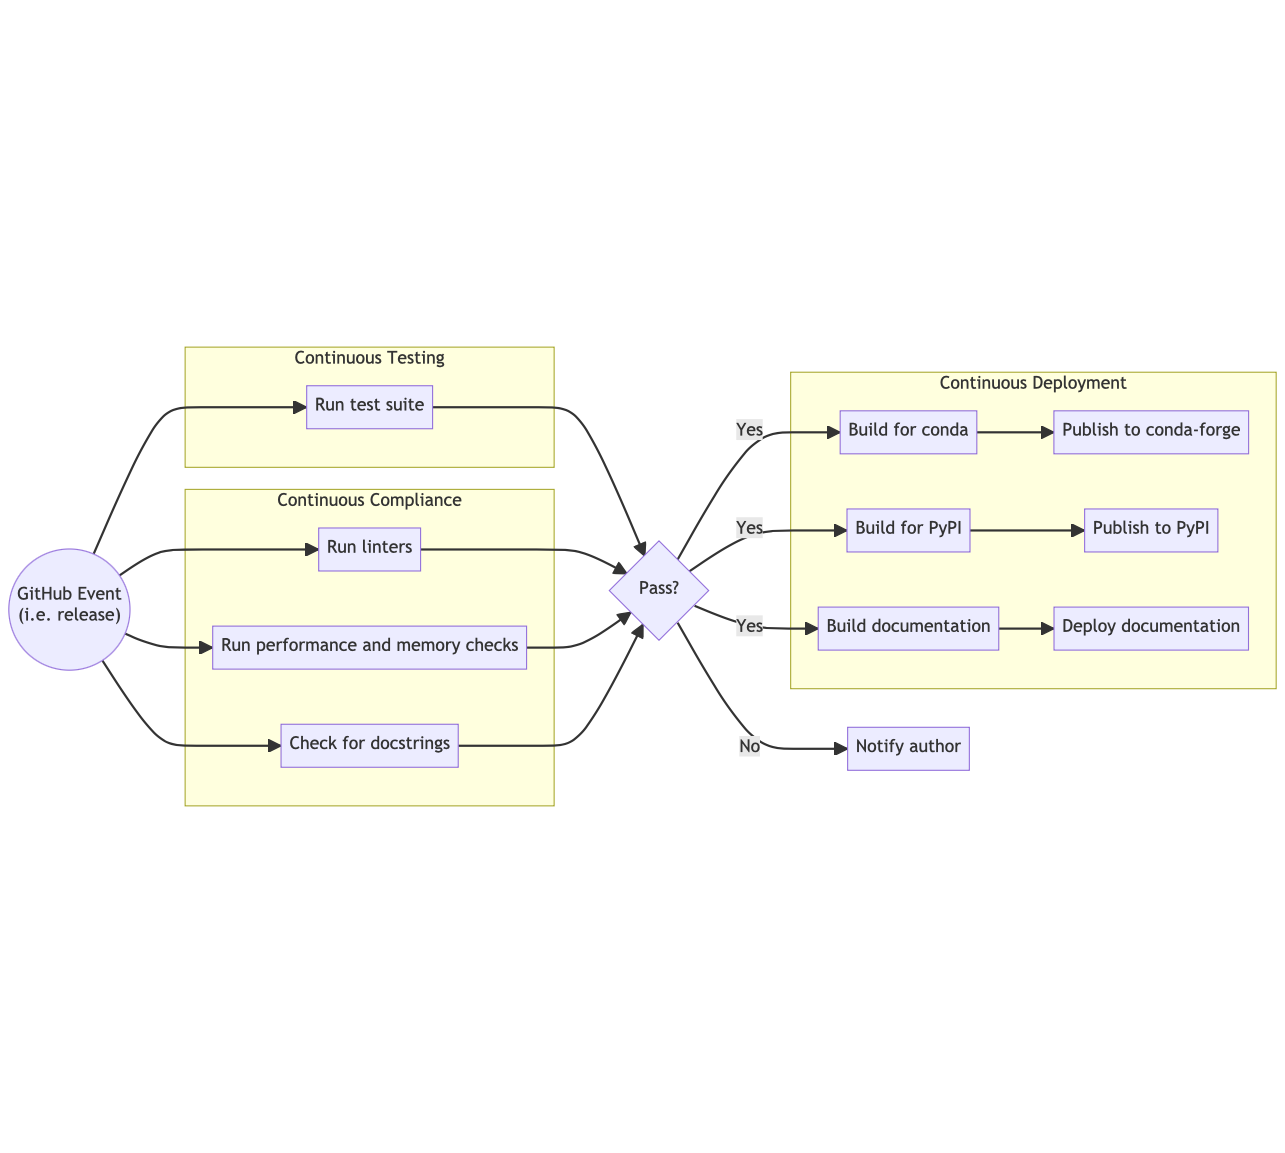
\includegraphics[width=0.7\textwidth]{mermaid-diagram-2023-10-02-133543.png}
\caption{A typical continuous integration (CI) pipeline using GitHub features including distinct steps for testing, compliance checking, and deployment.}
\label{fig:ci_pipeline}
\end{center}
\end{figure}


%%%%%%%%%%%%%%%%%%
% bibliography
%\cleardoublepage
%\label{sec:Bib}
%\nocite{*} %<--------- This command prints all entries in the bib file. Remove to cite only references cited in the report
%\printbibliography[heading=bibintoc, title={References}]


%%%%%%%%%%%%%%%%%%%%%%%%%%%%%%%%%%%%
\begin{appendices} %<--------- All chapters after this will be labeled as appendices
    
    % Reset the figure and table numbering to be A.1, etc.
    \counterwithin{figure}{chapter}
    \counterwithin{table}{chapter}

    \appchapter{RSE: The engineers behind research software}
    \label{app:A}

Research software exists in a unique environment where the majority of users and developers
share expertise within a specific field, and funding mechanisms are often tied to results
from using the software rather than to the software itself.
Because of these nuances of the research software environment, the incentives to create high
quality software are often misaligned with the career incentives for the engineers
creating the software.
Without the appropriate incentives, the best practices listed in this report will never gain
adoption, and WETO software will suffer in all of the areas listed.
For the sake of the WETO software portfolio and the researchers working in these groups,
it is important to directly consider the needs and expectations of the people
responsible for designing and implementing research software projects.

The term research software engineer (RSE) is defined by the
\href{https://society-rse.org/about/}{UK-RSE Society} as:

\begin{quote}
A Research Software Engineer (RSE) combines professional software engineering expertise with
an intimate understanding of research.
\end{quote}

While all modern research typically involves using research software, it is common for researchers
to focus skill development on either the research domain or the computational considerations
involved in implementing the research in software.
The research environments in academia and government labs are often structured to incentivize
academic publication, so the resulting teams are commonly made up of mostly domain researchers
and a minority of research software engineers.
The domain researchers inform the needs of the research software and are the primary users.
The RSE's design and develop the software systems as well as manage various IT responsibilities
for the group such as creating computer-based workflows, managing data, constructing web-based
research artifacts, and training colleagues on best practices in research computing.

In this context, note the difference between computer science and software engineering (both
descriptions taken from Wikipedia):
\begin{itemize}
\item \href{https://en.wikipedia.org/wiki/Computer_science}{Computer science} is the study of
    computation, information, and automation.
    Computer science spans theoretical disciplines (such as algorithms, theory of computation,
    and information theory) to applied disciplines (including the design and implementation of
    hardware and software).
    
\item \href{https://en.wikipedia.org/wiki/Software_engineering}{Software engineering} is an
    engineering-based approach to software development. A software
    engineer is a person who applies the engineering design process to design, develop, maintain,
    test, and evaluate computer software. The term programmer is sometimes used as a synonym,
    but may emphasize software implementation over design and can also lack connotations of
    engineering education or skills.
    Engineering techniques are used to inform the software development process, which involves the
    definition, implementation, assessment, measurement, management, change, and improvement of
    the software life cycle process itself.
\end{itemize}

\section{RSE value recognition}
Writing code and designing software systems are entirely different things, and the latter
must be recognized relative to the value that it adds to the research process.
Software design and software architecture are complicated topics covered in
\href{https://www.amazon.com/s?k=software+design&i=stripbooks&crid=2L9GNOIMWHMFD&sprefix=software+design%2Cstripbooks%2C166&ref=nb_sb_noss_2}{text books},
\href{https://web.stanford.edu/~ouster/cs190-winter23/}{courses at top universities}, and
\href{https://www.researchgate.net/search.Search.html?query=software+architecture&type=publication&subfilter%5BpublicationType%5D=article%2Fbook&subfilter%5BstartYear%5D=2022}{academic publications}.
The process of creating a software system given various requirements is a \textit{design process}.
It involves stating requirements, iterative design, and validation and verification of the design.
It can take years to fully accomplish a design objective, and at the same time the landscape of
computers and software development is constantly changing.
Additionally, software is rarely created by one person, so RSE's have to manage multiple
contributors making changes simultaneously while also striving to meet the needs of the project.
Therefore, consider it a best practice within the context of WETO software to recognize
the contributions and value of RSE's within the labs.
Avoid trivializing software design as "programming", and consider that many RSE's have engineering
or science degrees and treat their work as engineering or science.

\section{Career growth and trajectory}
In addition to acknowledgement of work and value added, it is important to provide meaningful
career guidance to RSE's to both serve their personal goals and ensure
that the projects have well-rounded contributors. RSE's should have some level of domain
experience; that is to say that they should \textit{use} as well as \textit{develop} their software.
RSE's should know the context in which their software exists.
They should be experts in the implementation and very good in the usage.
A characteristic career trajectory within the national lab environment may take the following path:

\begin{itemize}
\item Year 1: Implement models, develop tests and documentation
\item Year 2: Co-author analyses, improve modeling, inform AOP
\item Year 3: Lead author analyses, guide future development efforts, writing AOP
\item Year 4: Proposing new work, seeking funding to expand the software project
\item Year 5: Inform center-wide software culture and practices
\end{itemize}

In general, the amount of code written by a RSE should peak around year 2 or 3 and
then taper off. The responsibility for creating software should not be entirely removed, but
the majority of involvement in software development should be code review, design, and
project planning. As in any career advising, the details should be a discussion between RSE, their
direct manager, and the center or lab leadership.


\end{appendices}
%%%%%%%%%%%%%%%%%%%%%%%%%%%%%%%%%%%%

\end{document}



%%%%%%%%%%%%%%%%%%%%%%%%%%%%%%%%%%%%%%%%%%%%%%%%%%%%%%%%%%%%%%
%%%%%%%% Example figure, list, and table environments %%%%%%%%
%%%%%%%%%%%%%%%%%%%%%%%%%%%%%%%%%%%%%%%%%%%%%%%%%%%%%%%%%%%%%%

% %%% Example figure
% \begin{figure}[h] %<--------- placement options are (h)ere, (t)op, (b)ottom, (p)age. More than one option may be supplied.
%   \centering
%   \includegraphics[width=\columnwidth]{example-image-a} %<--------- path to graphics. Usually figures/<name of figure>
%   \caption[Optional short caption for LOF]{Actual caption for figure}
%   \label{fig:fig1}
% \end{figure}

% %%% Example subfigure
% \begin{figure}[h]
%   \centering
%   \begin{subfigure}[b]{0.48\columnwidth}
%     \includegraphics[width=\columnwidth]{example-image-b}
%     \caption{}
%     \label{fig:}
%   \end{subfigure}
%   \hfill
%   \begin{subfigure}[b]{0.48\columnwidth}
%     \includegraphics[width=\columnwidth]{example-image-c}
%     \caption{}
%     \label{fig:}
%   \end{subfigure}
%   \caption}
%   \label{fig:}
% \end{figure}

% %%% Example list
% \begin{itemize}
%   \item item 1
%   \item item 2
% \end{itemize}

% %%% Example table
% \begin{table}
%     \caption[Optional short table caption for LOT]{Actual table caption}
%     \label{tab:tab1}
%     \centering
%       \begin{tabular}{ccc}
%         \hline
%         a & b & c\\
%         d & e & f \\
%       \end{tabular}
% \end{table}

